\documentclass{article}

% Packages
\usepackage{titlesec}    % Customize section titles
\usepackage{lipsum}      % Generate dummy text
\usepackage{graphicx}    % Include images
\usepackage{caption}     % Customize captions
\usepackage{hyperref}    % Create hyperlinks
\usepackage{fancyhdr}    % Customize page headers and footers
\usepackage{geometry}    % Adjust page margins
\usepackage{authblk}     % Author and affiliation formatting
\usepackage{subcaption}
\usepackage{xcolor}
\hypersetup{
    colorlinks,
    linkcolor={red!50!black},
    citecolor={red!50!black},
    urlcolor={red!80!black}
}
\usepackage{natbib}      % Bibliography and citation management

% Page Margins
\geometry{margin=1in}

% Title Page
\title{Long-wave infrared sky images classification and probabilistic segmentation of cloud structures with deep-learning}
\author[1]{K. Sommer}
\author[2]{W. Kabalan}
\author[3]{R. Brunet}
\affil[1]{Laboratoire Univers et Particules de Montpellier, Université de Montpellier, CNRS, Montpellier, France; e-mail: \url{kelian.sommer@umontpellier.fr}}
\affil[2]{APC, Univ Paris Diderot, CNRS/IN2P3, CEA/lrfu, Obs de Paris, Sorbonne Paris Cité, France; e-mail: \url{wassim.kabalan@apc.in2p3.fr}}
\affil[3]{Laboratoire d’Astrophysique de Marseille, Marseille, France; e-mail: \url{romain.brunet@lam.fr}}
\date{\today}

% Section Title Formatting
\titleformat{\section}{\normalfont\Large\bfseries}{\thesection}{1em}{}
\titleformat{\subsection}{\normalfont\large\bfseries}{\thesubsection}{1em}{}
\titleformat{\subsubsection}{\normalfont\normalsize\bfseries}{\thesubsubsection}{1em}{}

% Page Header and Footer
\pagestyle{fancy}
\fancyhf{}
\rhead{\thepage}
\lhead{Long-wave infrared sky images classification and probabilistic segmentation of cloud structures with deep-learning}
\rfoot{K. Sommer, W. Kabalan and R. Brunet}

\begin{document}

\maketitle

\begin{abstract}
    Infrared thermal cameras offer reliable means of assessing atmospheric conditions by measuring the downard radiance from the sky, facilitating their usage in cloud monitoring endeavors. Precise identification and detection of clouds in images poses great challenges stemming from the indistinct boundaries inherent to cloud formations. Various methodologies for segmentation have been previously suggested. Most of them rely on color as the distinguishing criterion for cloud identification in the visible spectral domain and thus lack the ability to detect cloud structure on gray-scaled images with satfisactory accuracy. In this study, we present a complete deep-learning architecture performing image classification based on a Convolutional Neural Network (CNN) and image segmentation by exploring the use of the U-Net encode/decoder model. Our trained models effectively discriminate image types and capture precise cloud structure information even when trained with single ground truth per input sample. We conduct a series of tests and validation on self-captured and publicly available datasets. Results show that our method achieves better overall performance than other state-of-the-art methods. We emphasize our model architecture strong viability and accuracy for sustained cloud monitoring operations over extended durations through extensive validation experiments.\\

    \textbf{keywords}: ground-based cloud observation; thermal-infrared camera; cloud detection; deep-learning; image segmentation and classification; convolutional neural network; u-net
\end{abstract}

\section{Introduction}

% INTEREST OF CLOUDS IN GENERAL
Accurate and continuous monitoring of cloud properties contributes to a profound understanding of atmospheric processes and their subsequent impacts on various Earth systems \citep{liou1992radiation}. It provides essential insights for weather predictions and climate dynamics \citep{hu2004application, petzold2015global}.

% WAYS OF CLOUD OBSERVATION
Many diverse instruments are dedicated towards cloud detection and associated observation methods can be divided into two primary distinct categories: downward satellite-based observations and upward ground-based observations (e.g. all-sky cameras, lidar, radar). The principal aim of satellite-based observations is to investigate the upper regions of clouds, facilitating the examination and analysis of global atmospheric patterns and climate conditions over expansive geographical areas. In contrast, ground-based cloud observation excels in the surveillance of localized regions, furnishing valuable data pertaining to the lower segments of clouds (e.g. information on cloud altitude, cloud extent, and cloud typology).

% MORE ABOUT GROUND BASED OBSERVATIONS
Ground-based observations have been extensively used in recent years and has become one of the primary means to studying cloud formations \citep{paczynski2000monitoring}.As technological evolution has ushered in a new era of observation methodologies \citep{mandat2014all}, the utilization of infrared thermal cameras has emerged as a promising avenue for atmospheric investigations through precise radiometric measurements \citep{Szejwach1982, Shaw_2013, liandrat2017cloud, lopez2017contribution, Klebe2014, nikolenko2021infrared}.
%applications in many domains such as medicine \citep{ring2012infrared}, agriculture \citep{ishimwe2014applications}, military defence \citep{akula2011thermal} and surveillance systems \citep{wong2009effective}.
Because of their practical use, high sensitivity, low-cost, operating range and wide field-of-view (FOV), it makes them particularly useful for meteorological or even astronomical applications to determine the cloud cover fraction during operations and therefore assess the quality of scientific observations. Indeed, uncooled infrared microbolometers array sensors working in the 10-12 $\mu m$ spectral band can directly detect the LWIR emission of both clouds and the atmospheric background, excluding the scattered light of the sun or starlight \citep{Houghton1972}.
%Contrary to cameras operating in the visible spectrum, these LWIR sensors are able to provide reliable measurements of cloud properties at night. 
Across recent years, multiple automatic ground-based observations systems have been developed. For example, the infrared cloud imager (ICI) \citep{ICI}, can detect clouds and assess cloud coverage both in daylight and at nighttime with a dedicated infrared sensor. \citet{Sharma_2015} designed an instrument to detect of the cloud infrared radiations to be used in search for a potential site for India’s National Large Optical Telescope project.
%The ICI functions as a passive instrument, measuring the downward atmospheric radiance through a relatively narrow field of view (FOV) measuring about 250 deg$^{2}$ at a resolution of 320 $\times$ 240 pixels.
The all-sky infrared visible analyzer (ASIVA) \citep{Klebe2014} represents a distinctive device capable of acquiring an extensive field of view (FOV) infrared sky image without the need for a scanning mechanism. The ASC-200 system \citep{rs13091852} combines information from two all-sky cameras facing the sky operating in both the visible spectrum (450-650 nm) and the LWIR band (8-14 $\mu m$), called the TIRASVC instrument). It features a thermal microbolometer array sensitive to radiation in the 8–14 $\mu m$ spectral range and a specifically designed wide-angle germanium lens.

% RELATION TO ASTRONOMY
As next-generation cosmological surveys require more demanding precision on photometric observations (implying better characterization of the atmosphere), monitoring instruments field-of-view (FOV) with LWIR thermal cameras may provide significant asset to estimate cloud coverage, precipitable water vapor content (PWV) and classify observations quality. Multiple ground-based all-sky and narrow field-of-view (FOV) infrared instruments have demonstrated reliable measurements of sky radiance \citep{Klebe2012, Klebe2014}.
%For the upcoming Vera Rubin Observatory cosmological survey, preliminary work has demonstrated the feasability to monitor the entire sky with uncooled infrared cameras. 

In this study, we use a similar infrared sensor with a narrower FOV (i.e. 60 mm F1.25 germanium athermal lens) that aims to monitor a high-sensivity photometric telescope line of sight for astronomical purposes. It is part of the StarDICE metrology experiment \citep{stardice1} that aims at measuring CALSPEC \citep{Bohlin2014} spectrophotometric reference stars flux at the 0.1\% relative uncertainty level. Enhanced characterization of atmospheric conditions are required to reach the target sensitivity. As a first step, basic indication of the atmosphere conditions in the telescope FOV may provide valuable insights onto the quality of spectrophotometric measurements. However, these kind of instruments operate at high framerate and produce considerable amounts of data which make it extremely difficult to analyze by human observers. Therefore, to determine cloud presence in infrared images, deep convolutional neural networks appear to be a viable approach to process images in real-time. Inspired by large successes encountered in image classification and structure detection for various computer vision tasks, multiple models relying on convolutional neural network (CNN) have been developed, including: CloudSegnet \citep{dev2019cloudsegnet}, CloudU-Net \citep{CloudUNet} CloudU-Netv2 \citep{CloudUNetv2}, SegCloud \citep{SegCloud}, TransCloudSeg \citep{TransCloudSeg}, CloudDeepLabV3 \citep{CloudDeepLabV3}, ACLNet \citep{makwana2022aclnet}, DeepCloud \citep{DeepCloud}, CloudRaednet \citep{shi2022cloudraednet}, DMNet \citep{DMNet} and DPNet \cite{DPNet}.
Others are specifically dedicated toward satellite imagery \cite{kanu2020cloudx, chen2023novel}. Majority of these models are typically structured using an encoder–decoder architecture, with the encoder incorporating CNNs \citep{oshea2015introduction}. The encoder's role is to capture both high-level and low-resolution features, while the decoder generates the segmentation mask \citep{badrinarayanan2017segnet, Alzubaidi2021ReviewOD}. Nonetheless, these methodologies exclusively address RGB-colored images. Colors (or HUE) provides the essential of information for segmentation (especially red and blue channels). In the case of LWIR thermal images, we need to use a dedicated model capable of achieving comparable accuracy for single-channel gray-scaled images. Consequently, we develop a sequential deep-learning architecture designed to: (i) classify images (e.g, detect if any cloud is present onto the image); (ii) identify cloud structure (e.g., generate a probabilistic map) to verify if the CCD camera FOV is impacted.

In this paper, we propose two separate deep-learning models for classification based on standard Convolutional Neural Network (CNN) and U-Net encode/decoder network (e.g, consisting of convolution, deconvolution and pooling layers) for cloud structure identification. The first model discriminates between clear and cloudy images. The second provides a pixel-based semantic segmentation of images in the form of a probability map.

The main contributions of this paper are:
\begin{itemize}
    \item DeepCloud: a novel ground-based cloud image feature
    extraction approach based on deep learning. It first intro-
    duces the multiple convolutional layers within CNN to
    characterize the cloud image;
    \item FV encoding is applied to addressing the multi-instance
    learning problem within cloud image categorization that
    cannot be well handled by CNN;
    \item  A discriminative pattern mining  approach is proposed to
    discard the local confusing cloud patterns.
\end{itemize}

The source code and supporting materials of DeepCloud are
published on https://github.com/liangye518/DeepCloud.

The remainder of the paper is organized as follows. The experimental setup and data acquisition procedure are detailed in Section 2. Model architectures principles and algorithms of cloud identification and structure detection are described in Section 3. Results and relevant discussions are presented in Section 4. Section 5 shows a summary of the conclusions.

\section{Related work}

In recent years, numerous cloud sky/cloud segmentation algorithms have been introduced along with the increased development of all-sky ground-based cloud monitoring stations \citep{RetrievingCloudCharacteristicsfromGroundBasedDaytimeColorAllSkyImages, rs12111902, ASC2, amt-15-3629-2022}.
Indeed, cloud segmentation is big challenge for remote sensing applications as cloud comes in various shapes and forms. Therefore, the most modern common approach aims to use computer vision encoder-decoder architectures algorithms and train them onto very specific publicly available cloud images database such as: SWIMSEG, SWINSEG, SWINySEG (combination of both), WSISEG, HYTA and TLCDD. Most proposed solutions are focus on visible RGB images.
CloudSegNet \citep{dev2019cloudsegnet} is a light-weight deep-learning encoder/decoder network that detects clouds onto daytime and nighttime visible color images.
CloudU-Net \citep{CloudUNet} modifies CloudSegNet architecture by adding dilated convolution, skip connection, and fully connected conditional random field (CRF, see \citealt{McCallumCRF}) layers to demonstrates better segmentation performance overall. It uses the powerful U-Net architecture \citep{UNET} originally applied to medical image segmentation.
CloudU-Netv2 \citep{CloudUNetv2} replaces the upsampling in CloudU-Net with bilinear upsampling, improves discrimination ability of features representation and uses rectified Adam (rADAM is a variant of the Adam \cite{ADAM} stochastic optimizer that introduces a term to rectify the variance of the adaptive learning rate, see \citet{RADAM}) as the optimizer.
SegCloud \citep{SegCloud} has been trained onto 400 images and possesses a symmetric encoder–decoder structure and outputs low/high-level cloud feature maps to the same resolution of input images.
TransCloudSeg \citep{TransCloudSeg} adresses the loss of global information due to limited receptive field size of the filters in CNN by proposing an hybrid model containing both the CNN and a transformer \citep{TRANSFORMER} as the encoders to obtain different features.
CloudDeepLabV3+ \citep{CloudDeepLabV3} designs a lightweight ground-based cloud image adaptive segmentation method  that integrates multi-scale fea­tures aggregation and multi-level attention feature enhancement.
ACLNet \citep{makwana2022aclnet} uses EfficientNet-B0 as the backbone, “à trous spatial pyramid pooling” (ASPP see \citet{ATROUS}) to learn at multiple receptive fields, and “global attention module” (GAM see \citet{GAM}) to extract fine-grained details from the image. It provides lower error rate, higher recall and higher F1-score than state-of-art cloud segmentation models.
DeepCloud \citep{DeepCloud} uses the method of Fisher vector encoding which is applied to executing the spatial feature aggregation and high-dimensional feature mapping on the raw deep convolutional features.
CloudRaednet \citep{shi2022cloudraednet} proposes a residual attention-based encoder–decoder network and train it over the SWINySEG dataset.
\citep{MACNN} introduces a novel deep model named multiscale attention convolutional neural network (MACNN) to obtain different receptive fields by using different hole rates for the filters and propose the attention module to learn the attention coefficients in order to reflect different importance of pixels.
DMNet \citep{DMNet} proposes a novel cloud detection network that aims to achieve information complementarity by exploiting the different properties of the features at different levels of the encoder, so as to strengthen the detailed information of high-level features and make the low-level features have more semantics.
DPNet \citep{DPNet} possesses an encoder-decoder structure
with Dual Pyramid Pooling Module (DPPM). Specifically, they process the feature maps of different scales in the encoder through a technique known as dual pyramid pooling. They also implement the Encoder-Decoder Constraint (EDC) to relieve information loss in the process of encoding and decoding.

Overall, the primary innovation brought forth by CNN-based approaches in the realm of ground-based cloud image segmentation is the introduction of the encoder–decoder architecture. The encoder is tailored to acquire representational features, facilitating the extraction of semantic information. Subsequently, the decoder reconstructs these representational features into the segmentation mask, allowing for pixel-level classification.

Others have proposed solutions for all-sky infrared image classification. \citet{CloudClassificationBasedonStructureFeaturesofInfraredImages} applies pre-processing steps (smoothing noise reduction, enhancement through top-hat transformation and a high-pass filtering, edges detection) before extracting features that are useful for distinguishing cirriform, cumuliform, and waveform clouds. A simple rectangle method as supervised classifier is applied. They find a 90\% agreement between a priori classificatoin carried out manually by visual inspection and their algorithm on 277 images. \citet{SUN2011278} suggested: (i) a method for determining clear sky radiance threshold; (ii) cloud identification combined threshold method with texture method; (iii) an algorithm to retrieve cloud base height from downwelling infrared radiance. They showed that structural features are better than texture features in classifying cloud. \citet{amt-11-5351-2018} proposed a three-step process: (i) pre-processing; (ii) feature extraction; (iii) classification method to group images into five cloud categories (stratiform, cumuliform, waveform, cirriform and clear) based on manifold and texture features using support vector machine (SVM). Their experimental results demonstrate the higher recognition rate with an increase of 2\%–10\% on ground-based infrared images datasets. Nevertheless, these methods class clouds into separate categories based on their typology.
In this paper, we present a new framework based on CNNs and U-Net based algorithms to identify cloud images and detect cloud structure in real-time.


%\citet{ASC2} developed an automatic all-sky imaging system (ASC), for cloud cover evaluation. They also introduced a dedicated cloud detection algorithm relying on an optimized U-Net model.

\section{Methodology}

In this section, we outline the architectural designs of two distinct deep-learning models tailored for cloud-related tasks. On the one hand, we implement a classifier for cloud classification using Convolutional Neural Networks (CNN), whose only goal is to discriminate between cloud-free and cloudy images. On the other hand, the segmentation for cloud structure detection is performed via the U-Net model. The output probability map can later be thresholded according to the user needs in order to produce the desired predicted binary segmentation map.

Both architectures are implemented in \textsc{Python} with the \textsc{keras}\footnote{\url{https://keras.io}} subpackage of \textsc{TensorFlow}\footnote{\url{https://www.tensorflow.org}} framework\footnote{The code developed in this paper is freely available online at \url{https://github.com/Soumyabrata/CloudSegNet}.}. Images are normalized and binned into a fixed 160 $\times$ 128 resolution format to speed up computations and to capture the global trend. Models are trained over 500 and 1000 epochs respectively using the ADAM optimizer. We use batch of 16 images with dynamic learning rate of 0.001 that decreases through the training epochs. Hyperparameters are fine tuned with the \textsc{optuna}\footnote{\url{https://optuna.org/}} hyperparameter optimization framework.

\subsection{Image classification}

Our classification model architecture consits of a Convolutional Neural Network (CNN) architecture for the purpose of distinguishing between infrared images containing clouds and those that are cloud-free. The CNN architecture consists of multiple layers designed to extract and learn relevant features from the input images. The model commences with a series of convolutional layers, each followed by rectified linear unit (ReLU) activation and max-pooling operations. This configuration facilitates the extraction of hierarchical features that are pivotal for accurate classification.

The output of the convolutional layers is then flattened and fed into fully connected layers, culminating in a final softmax layer for cloud classification. To prevent overfitting, dropout layers are strategically incorporated during training. The model is trained on a comprehensive dataset encompassing both cloud and cloud-free infrared images, with corresponding ground truth labels. The categorical cross-entropy loss function is employed for optimization, aiming to minimize the discrepancy between predicted and actual classifications.

\begin{figure}[!h]
	\includegraphics[width=\hsize]{figures/FLOWCHARTS_DL_IR.pdf}
	\caption{
		Schematic diagram of the U-net encoder/decoder model architecture to identify cloud structures. Boxes represent cross-sections of square feature maps. Each map's dimensions are indicated on its lower left, and its number of channels are indicated above it. Half-grey boxes represent maps for which half of their channels are copied. The input image is a 160 × 128 radiometrically calibrated grayscale image of the sky from the LWIR instrument. Classifier model output is a boolean. Arrows represent operations, specified by the legend-notably, blue arrows represent convolutions, while gray ones represent copying (skip connections). Tensor dimensions at the output of each block are specified.  \label{fig1}}
	\end{figure}
	\unskip

\subsection{Image segmentation}

For cloud structure identification, the U-Net architecture is adopted owing to its effifiency in semantic segmentation tasks. The U-Net model comprises an encoder and a decoder, facilitating the capturing of context-rich features and precise delineation of cloud structures. The encoder integrates convolutional and max-pooling layers to progressively downsample the input image, thereby capturing high-level features. These features are then decoded using up-convolutions and skip connections, enabling the reconstruction of the segmented cloud structures. Figure \ref{} shows the architecture of the model.

\begin{figure}[!h]
    \centering
    
    \begin{subfigure}{\textwidth}
        \centering
        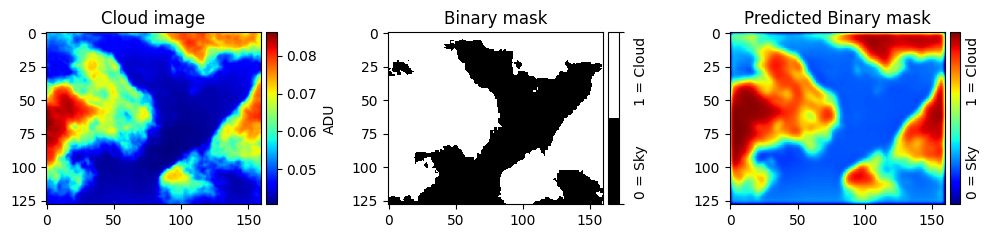
\includegraphics[width=1.0\linewidth]{figures/test_dl_15epochs.png}
        \label{fig:sub1}
    \end{subfigure}
    
    \begin{subfigure}{\textwidth}
        \centering
        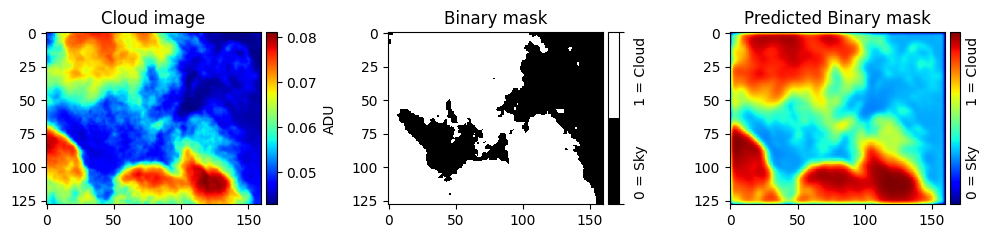
\includegraphics[width=1.0\linewidth]{figures/test_dl_15epochs2.png}
        \label{fig:sub2}
    \end{subfigure}
    
    \begin{subfigure}{\textwidth}
        \centering
        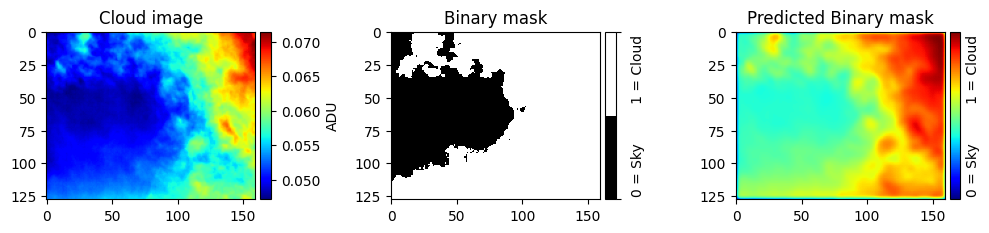
\includegraphics[width=1.0\linewidth]{figures/test_dl_15epochs3.png}
        \label{fig:sub3}
    \end{subfigure}

    \caption{Overall caption for the figure containing three plots.}
    \label{fig:all}
\end{figure}

\begin{figure}[!h]
	\includegraphics[width=10.5 cm]{figures/FLOWCHARTS_DL_IR.pdf}
	\caption{
		Schematic diagram of the U-net encoder/decoder model architecture to identify cloud structures. Boxes represent cross-sections of square feature maps. Each map's dimensions are indicated on its lower left, and its number of channels are indicated above it. Half-grey boxes represent maps for which half of their channels are copied. The input image is a 160 × 128 radiometrically calibrated grayscale image of the sky from the LWIR instrument. The output image is a probabilistic mask prediction of pixels being cloudy or clear. Arrows represent operations, specified by the legend-notably, blue arrows represent convolutions, while gray ones represent copying (skip connections). 	Tensor dimensions at the output of each block are specified. Classifier model output is a boolean. \label{fig1}}
	\end{figure}
	\unskip

\subsubsection{Encoder block}

The encoder block of CIRRUS identification model consists of four convolution layers and four max-pooling layers. We feed a normalized and binned 4x4 radiometrically calibrated image of a fixed input size (160 × 128 pixels) into the model.
The initial convolutional layer applies a set of learnable filters to the input image, extracting low-level features. Additional convolutional layers increase the complexity of learned features by applying convolutions to the feature map generated by the previous layer, creating a hierarchy of increasingly abstract features. After a set of convolutional layers, a max-pooling layer is applied to downsample the feature map. Max-pooling helps to reduce the spatial dimensions of the feature map while retaining the most salient information.

\subsubsection{Decoder block}

The decoder takes the high-level features generated by the encoder and aims to restore the spatial resolution of the original input image. In the U-Net architecture, the decoder is connected to the encoder via skip connections, enabling the network to combine local and contextual information. The decoder starts with an upsampling operation to increase the spatial dimensions of the feature map. A skip connection connects the upsampled feature map from the decoder with the corresponding feature map from the encoder. This enables the network to leverage both local and global context information. Following the concatenation, a series of convolutional layers are applied. These layers refine the combined feature map, gradually transitioning from abstract features to more detailed information. The final convolutional layer produces the segmentation mask of the U-Net model.

\subsubsection{Loss function}

The U-Net model is trained on labeled datasets containing infrared images with pixel-wise cloud structure annotations. The loss function employed for training is typically the binary cross-entropy, which quantifies the difference between predicted probabilities and actual binary class labels for each instance in the dataset. Mathematically, given an instance's true binary label $y$ (0 or 1) and the predicted probability $p$ of it belonging to class 1, the binary cross-entropy loss $\mathcal{L}$ is calculated as:
\begin{equation}
	\mathcal{L} = -\frac{1}{N}\sum_i y_i\cdot\log\left(f_w(x_i)\right) + (1-y_i)\cdot\log\left(1-f_w(x_i)\right)
\end{equation}
where $\mathcal{L}$ is the binary cross-entropy loss. $N$ is the total number of instances in the dataset, $i$ index represents an individual instance, $y_{i}$ is the $i$-th true binary label (0 or 1) and $f_w(x_i)$ is the predicted probability that belongs to class 1, based on the model with parameters $w$.
The goal of training is to minimize this loss function by adjusting the model parameters weights $w$ to better align the predicted probabilities $f_w(x_i)$ with the true labels $y_{i}$.

\subsubsection{Model output}

The output the classifier is a boolean representing whether the image contains cloud or not. On the contrary, the image segmentation model output is a probability mask that assigns a probability value to individual pixels, indicating their potential belonging in the cloud category.
 %Subsequently, a straightforward thresholding technique is applied to transform the probability mask into a binary map. The threshold for labeling is obtained from the Receiver Operating Curve (ROC) analysis specific to our experimental conditions.

\section{Experimental setup and dataset}

\subsection{Description of the instrument}

Our instrument is a FLIR Tau2 infrared thermal camera operating in the 8-14 $\mu m$ LWIR band. It consists of a focal plane array (FPA) of 640 $\times$ 512 uncooled microbolometers with 9 Hz framerate. The sensor is coupled with a narrow FOV thanks to the 60 mm F1.25 lens. The major goal of installing it on the equatorial table next to the photometric telescope of the StarDICE experiment is to evaluate sky conditions in the visible CCD camera line of sight at any instant during observations. With careful calibration, radiative transfer and simulations data analysis, we can extract useful properties of the sky to assess the atmospheric condition in real-time. Figure \ref{} shows the instrument mounted with the required controlling equipment onto the equatorial table facing the zenith inside the observatory dome. Surrounding and camera internal temperatures are monitored in real-time to correct for temperature-dependent fluctuations of the sensor response. Device control/command and image acquisition is done with the ThermalCapture ThermalGrabber USB 2.0\footnote{\url{https://thermalcapture.com/thermalcapture-grabber-usb-2-0-documents/}} interface allowing makes access to full 14-bit radiometric raw data. We develop an in-house \texttt{Python} program to control functionalities and grab images from the camera available on GitHub in open-access\footnote{\url{https://github.com/Kelian98/tau2_thermalcapture}}. Images are written into \texttt{FITS} files. An improved flat-field calibration source is positioned at regular intervals of $\approx$ 30 seconds to correct for anisotropies in pixel responses to due fixed pattern noise (FPN). True scene radiances are computed from raw images with per pixel calibration coefficient matrices (see \ref{}).

\begin{figure}
    \centering
    
    \begin{subfigure}[b]{0.4\textwidth}
        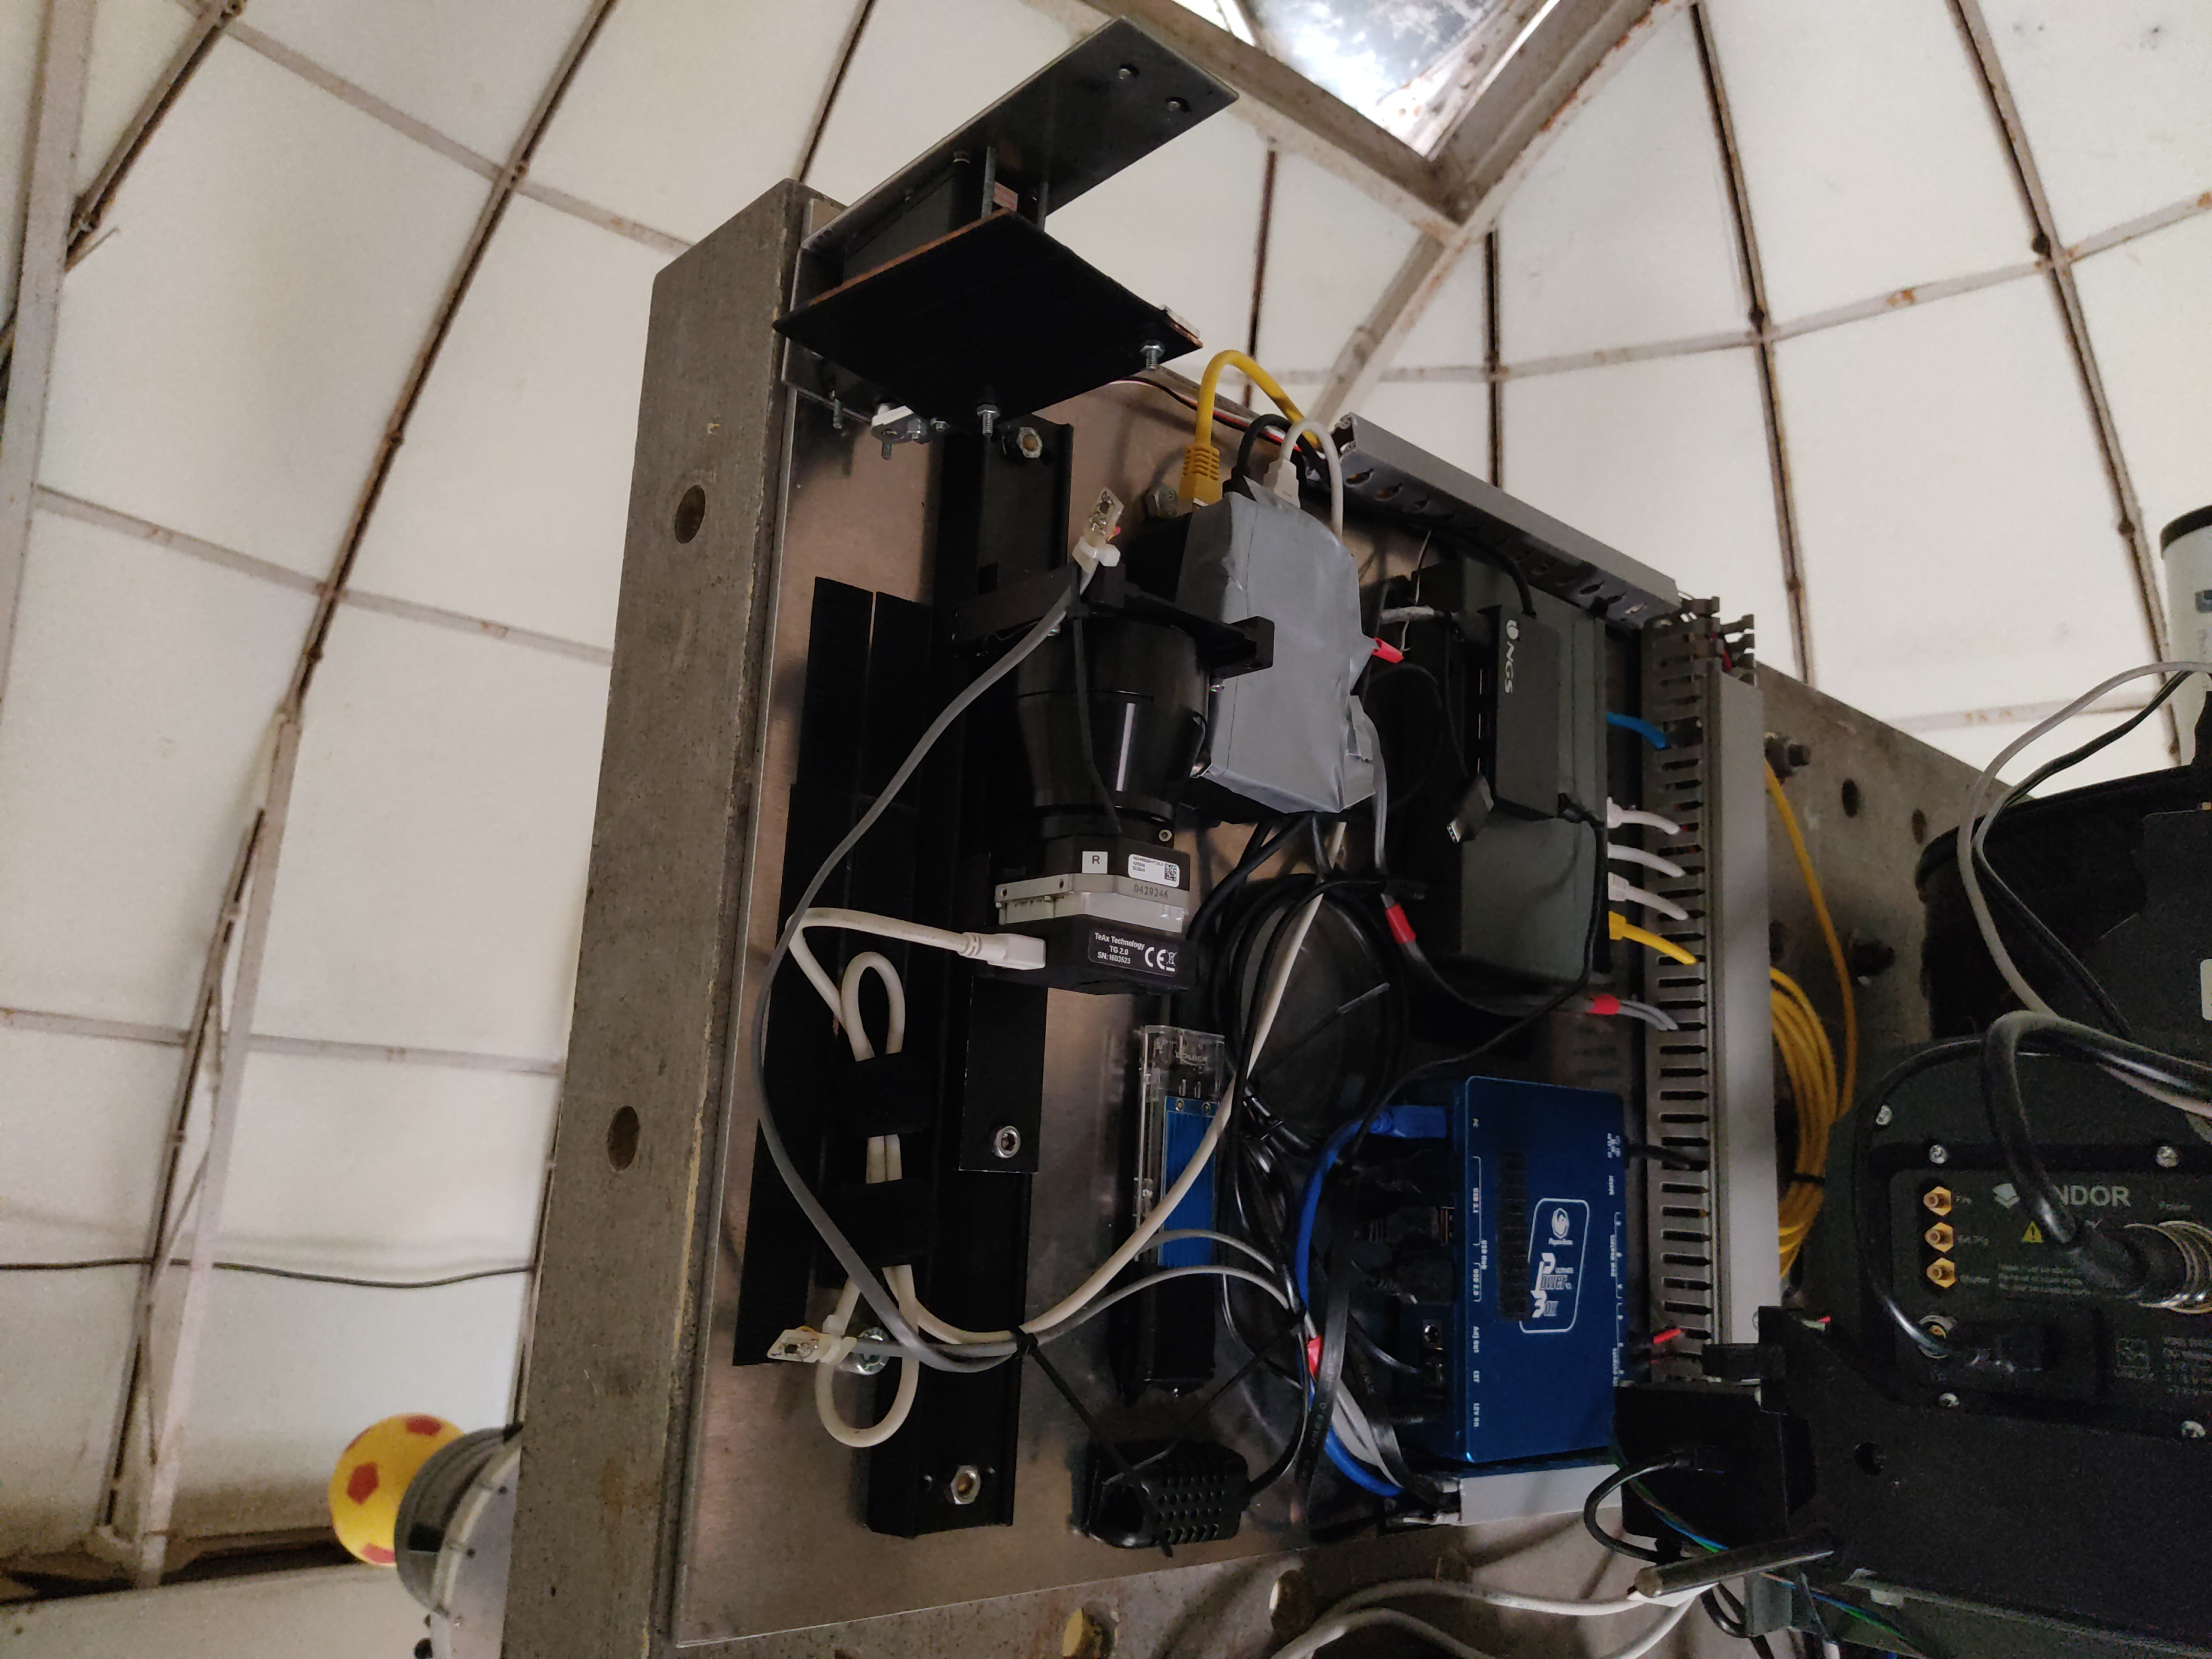
\includegraphics[width=\textwidth]{figures/infrared_instrument.jpg}
        %\caption{Subfigure 1}
        \label{fig:subfig1}
    \end{subfigure}
    \hfill
    \begin{subfigure}[b]{0.5\textwidth}
        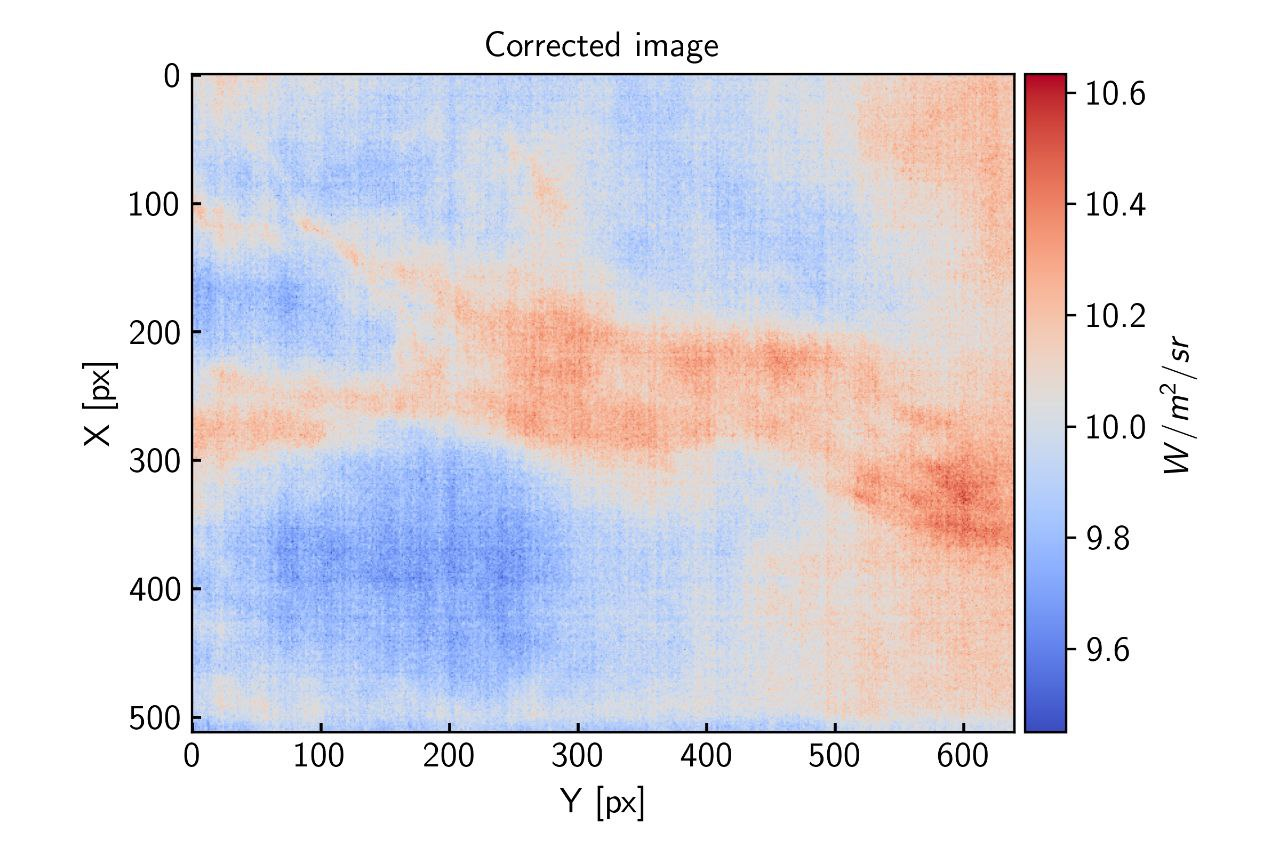
\includegraphics[width=\textwidth]{figures/calibrated_sky_image.jpg}
        %\caption{Subfigure 2}
        \label{fig:subfig2}
    \end{subfigure}
    
    \caption{\textit{Left:} infrared instrument installed onto the equatorial table of the StarDICE experiment at Observatoire de Haute-Provence. \textit{Right:} sample of radiometrically calibrated image.}
    \label{fig:side_by_side}
\end{figure}


%\subsection{Extraction of sky/cloud data from LWIR images}

%Infrared radiation has been recognized as holding significant promise in yielding valuable insights into cloud properties and atmospheric information. The 8–14 $\mu m$ spectral range - specifically the 10-12 $\mu m$ sometimes called the \textit{transparency window} - is characterized by minimal atmospheric emission and absorption. Radiative simulations of the atmosphere with \textsc{libRadTran} can provide a clearer depiction of the atmospheric window's attributes (e.g, sky downwelling radiance spectrum, transmittance, emittance). Figure \ref{} illustrates one typical simulation with different atmosphere reference models in the LWIR. Curves may be shifted up or down as a function of the zenith angle $\theta_{z}$, the total quantity of ozone $O_{3}$, the precipitable water vapor (PWV) or the vertical aerosol optical depth (VAOD). We can denote high atmospheric transmittance and low atmospheric emission, apart from a region around 9.6 $\mu m$ due to ozone (O3) absorption.

%Sky radiance emitted by the atmosphere is primarily controlled by water vapor content and clouds. During clear-sky/cloud-free conditions, the radiation received at the ground is both minimal and subject to fluctuations based on the quantity of water vapor present. Previous investigations have demonstrated a quadratic relationship between downwelling infrared radiation and the amount of precipitable water vapor (PWV). 

\subsection{Dataset and pre-processing}

Our dataset consists of 160 $\times$ 128 images which have been binned in 4$\times$4 format from the original large resolution of 640 $\times$ 512. Cloudy sky images were collected over a period of 3 nights at Observatoire de Haute-Provence in January 2023 (43° 55' 51" N, 5° 42' 48" E). Cloud-free images were collected over a short period of time during the same month. However, to compensate the lack of cloud-free images and prevent any bias during training due to the data imbalance, we generate synthetic cloud-free images to form a composite cloud-free dataset containing as much images as the cloudy dataset. Synthetic images reproduce realistic observations by generating 2D horizontal gradient based images simulating increase in sky downwelling radiance as the camera FOV tilts towards high zenith angles (i.e, low elevation angles). Realistic sources of noises affecting uncooled infrared thermal cameras are introduced, including: read noise, fixed pattern noise, sky noise and narcissus effect. These are added so that the image spatial noise is equivalent to true cloud free images. Figure \ref{} depicts one typical cloud-free image and a synthetic generated one with the spatial noise denoted for each of them. Note that the absolute ADU value has no impact as data is normalized prior to training.

Ground-truth masks identifying cloud structure on cloud images were manually created through multiple steps of stretching procedures using \textsc{astropy} methods. They consist of boolean 2D array of the same image size, where \textit{True} identified pixels represent cloud pixels and \textit{False} identified pixels represent clear sky areas. This step could not be automated as cloud optical depths differ significantly. Indeed, the segmentation model aims at automating this tedious time consuming operation in real-time during observations. Figure \ref{} depicts two raw images with their associated manually generated ground-truth cloud masks for training purposes.

All images and masks are visually inspected. Samples presenting artifacts such as tree branches from surroundings or building in the corner FOV are discarded. As the camera acquisition framerate enables to record up to 9 images per second, the pre-processing algorithm included constraints on consecutive image selection based on their timeseries. Selected frames are taken from at least 2 seconds between each other.

Moreover, we performed multiple random augmentations (e.g, flip, shear, rotate, shift and zoom) on each original image to double the size of each dataset. All augmented images are produced through the random sequential applications of these five distinct operations to initial images. After the selection and augmentation procedures, we conducted a visual examination of all the created sky/cloud images to ensure that they appear realistic. Since all the parameters in the image augmentation process undergo controlled adjustments, our generated images closely mirror authentic sky/cloud scenes.

Datasets are for both models are splitted into training, testing and validation subsets with ratio of in the ratio of 70\%, 20\% and 10\% respectively.

\section{Results}

\subsection{Loss-trend of CIRRUS}

We use this augmented composite datasets of 10,000 images respectively to train the classifier and identifer. Random sampling is applied on each composite dataset, and standard train-test-validation split is perormed . Figure \ref{} depicts trends for the binary cross-entropy losses for training and testing subsets with various hyperparameters. \textsc{Optuna} framework allows ease of hyperparameters optimization. We observe that the loss saturates after a few hundred iterations for all attempts, and the model exhibits comparable loss performance for both training and testing sets. We select the model and layer parameters with the lowest validation loss for our subsequent experiments.

\subsection{Performance}

We use multiple quantitative metrics to evaluate our segmentation model : completeness, purity, Intersection over Union (IoU), precision, recall, F-score and Error Rate between the ground-truths and the predictions.

Results are summarized in Table \ref{}. The purity is also
very high, with a value of 98.5. For classificatoin, the model reaches high performance of XXX accuracy and XXX YYY. We measure a completeness of 87 and a purity of 93.6. Our cloud structure identification model reaches an IoU above 0.8 at any magnitude, and up to 0.9 for bright objects (small magnitude).

\section{Results}


\section{Discussion}
Summarize the key points of your article and state your conclusions.


\section{Conclusion}
Summarize the key points of your article and state your conclusions.

\section*{Acknowledgments}
You can acknowledge any individuals or organizations that supported your research.

\bibliographystyle{unsrt}
\bibliography{biblio}

\end{document}
